% Giới thiệu


% Giới thiệu

\chapter{Giới thiệu}
Hiện nay một cuộc cách mạng về công nghệ đang bắt đầu, nó bắt nguồn từ những thành tựu nổi bật đạt được trong lĩnh vực trí tuệ nhân tạo (Artificial Intelligence hay AI) ở vài năm trở lại đây. Sự tác động của AI đang góp phần chuyển đổi mọi mặt đời sống, xã hội từ các ngành công nghiệp như tự động hóa, giao thông, liên lạc, nông nghiệp công nghệ cao.. cho đến giáo dục, y tế, chăm sóc sức khỏe...\\

  AI đã nhen nhóm phát triển từ những năm 70 của thế kỉ XX, sau đó đã chững lại một thời gian cho đến khi Geofrey Hinton công bố bài báo \cite{GeoffHinton2006} về cách huấn luyện một mạng neuron có khả năng nhận biết các con số viết tay với độ chính xác là hơn 98\%, họ đã mô tả kĩ thuật này là deep learning (học sâu). Nhưng thực ra nó là một mạng neuron nhân tạo (Artificial Neural Network) đây là một giải thuật học của học máy (Machine Learning) nhằm mô hình hóa lại khả năng học của não người.
Từ kết quả của Geoffrey, các nhóm nghiên cứu sau đó đã cho ra đời nhiều mô hình Covolutional Neural Network (CNN) mới như AlexNet\cite{Krizhevsky2012} , VGGNet\cite{Simonyan2014}, ResNet\cite{KHe2015} được biết đến qua cuộc thi ImageNet Large Scale Visual Recognition Challenge (ILSVRC). Những mô hình này không những đạt được kết quả tốt với bài toán phân loại ảnh (image classification) mà còn cải thiện kết quả của các bài toán khác như nhận diện vật thể  (object detection), phân đoạn đối tượng (instance segmentation) một cách vượt trội. Nhận ra được tiềm năng mà các mô hình kể trên mang lại, các nhóm nghiên cứu về AI đang tìm cách áp dụng nó để giải quyết các bài toán mà họ đang theo đuổi.\\

Ở đề tài này nhóm cũng sẽ tận dụng những kết quả trên để giải quyết một vấn đề rất cơ bản trong thị giác máy tính đó là bài toán ước lượng độ sâu từ ảnh (depth estimation) hoặc dự đoán độ sâu (depth prediction) và dùng nó để ước lượng khoảng cách từ camera đến vật thể trong ảnh. Ước lượng độ sâu là bài toán dự đoán khoảng cách tại mỗi điểm ảnh của một bức ảnh RGB, nó có nhiều ứng dụng quan trọng và rộng rãi trên nhiều lĩnh vực như rô-bốt (robotics), hiểu khung cảnh (sence understanding), xe tự lái (autonomous driving), thực tế ảo (augmented reliaty hay AR), phục hồi 3-D (3-D reconstruction).... Mặc dù trên thị trường hiện nay có nhiều cảm biến để đo độ sâu như Kinect... hoặc LiDAR, máy ảnh stereo, nhưng bọn chúng đề có hạn chế riêng. Cụ thể, một cảm biến 3D LiDAR tốt có chi phí cực cao, còn các loại cảm biến tương tự như Kinect thì không cho kết quả tốt khi ở ngoài ánh sáng mặt trời và tiêu thụ nhiều năng lượng. Cuối cùng với máy ảnh stereo nó dùng một cặp ảnh để tính toán nhằm ước lượng khoảng cách nên đòi hỏi chi phí tính toán cao và thường thất bại tại những vùng không có đặc trưng nổi bật. Do đó từ những hạn chế trên nên nhóm cực kì hứng thú với kĩ thuật ước lượng độ sâu sử dụng một máy ảnh kĩ thuật số bởi vì nó nhỏ, nhẹ, chi phí thấp, tiết kiệm năng lượng và là loại hàng điện tử phổ biến nhưng đây cũng là vấn đề có nhiều thách thức đặt ra, cụ thể  như, khi ta chụp một bức ảnh trong môi trường indoor thì các vật thể bị che lấp với nhau, bề mặt lồi lõm, biến đổi phức tạp, tất cả điều này gây ảnh hưởng rất lớn đến kết quả ước lượng độ sâu. Đồng thời chỉ với một bức ảnh 2D thông thường có thể có vô số khung cảnh trong không gian 3 chiều tương ứng với nó. Dĩ nhiên đa số chúng không hợp lí trong không gian thực, nên độ chính xác của độ sâu mà ta dự đoán vẫn có thể đạt độ chính xác cao. Mặc dù chúng ta biết rằng, đối với con người thì việc nói chính xác giá trị khoảng cách của một điểm cụ thể tại một không gian cụ thể đã là điều rất khó, chúng ta chỉ có thể  nói giá trị đó thuộc khoảng nào thôi. Cho nên vấn đề này đối với máy tính lại càng thách thức hơn nữa.\\

%% phía trên ở đề tài, chỗ này cugnx ở để tài.
Do đó ở đề tài này nhóm đã thực hiện nhiều khảo sát, nghiên cứu trong và ngoài nước để đưa ra một mô hình có độ chính xác cho phép, để có thể áp dụng vào thực tiễn. Sau khi chọn được mô hình ước lượng độ sâu phù hợp nhóm sẽ tiến hành hiện thực và tùy chỉnh mô hình. Kết thúc giai đoạn ước lượng độ sâu chúng ta sẽ có giá trị khoảng cách từ camera đền mỗi điểm ảnh tương ứng. Để ước lượng khoảng cách, ở giai đoạn này nhóm sẽ chọn một framework phổ biến để nhận diên vật thể, sau đó kết hợp với giá trị độ sâu ở giai đoạn trước, nhóm sẽ đưa ra một vài phương pháp để có thể xấp xỉ khoảng cách từ camera đến các vật thể nhận diện được trong bức ảnh RGB.\\

\begin{comment}
Sau đây là những công việc cụ thể mà nhóm đề ra nhằm hoàn thành đề tài.
\begin{itemize}
	\item Phân tích đề tài: Nhằm hiện thực được các bài toán đề ra. Nhóm cần tìm hiểu và sau đó làm chủ những kiến thức nền tảng và kĩ thuật liên quan mà đang được sử dụng hiện nay.
	\item Dữ liệu: Ở giai đoạn ước lượng độ sâu (depth estimation) bọn em dùng kĩ thuật học sâu, nên điều tối quan trọng ở giai đoạn này là cần có tập dữ liệu (data set) để huấn luyện mô hình. Nhóm sẽ tìm kiếm và chọn ra những tập dữ liệu phù hợp để khi kết thúc quá trình huấn luyện, mô hình cho ra những kết quả tiên đoán như mong muốn.
	\item Chọn lựa và hiện thực mô hình: Nhóm sẽ tiến hành khảo sát các công trình liên quan.
  Đánh giá, so sánh ưu và nhược điểm của các mô hình đồng thời xem xét năng lực của nhóm cũng như tài nguyên hiện có để chọn ra và hiện thực lại mô hình.
   \item Đánh giá mô hình: 
   Nhóm sẽ tìm hiểu những thước đo phổ biến mà các nhóm nghiên cứu dùng để xem xét chất lượng của kết quả mà mô hình tạo ra. 
   \item  Tiến hành ước lượng khoảng cách và so sánh kết quả của những phương pháp : Bước vào giai đoạn sau nhóm sẽ chọn ra một framework để nhận diện vật thể
   cùng với kết quả có được ở giải đoạn đầu nhóm sẽ tiến hành ước lượng khoảng cách của những vật thể nhận diện được thông qua những phương pháp ước lượng do nhóm đề xuất. Cuối cùng nhóm sẽ tiến hành so sánh những kết quả đó và nhau và đưa ra được độ tin cậy của chúng.
   
\end{itemize}
\end{comment}


% giống văn liệt kê quá, không cần biết là 7 chương.  TIếp theo đây... cũng được. Đừng ghi kiểu: chương 1 ..., chương 2 ... Đổi thành chương 1... Sau đó nhóm thực hiện ... ở chương 3 và 4. ....

Báo cáo của nhóm gồm 7 chương. Sau chương này, nhóm sẽ trình bày những khảo sát, tìm hiểu về những công trình liên quan về  bài toán ước lượng độ sâu và nhận diện vật thể. Chương tiếp theo sẽ nói về những kiến thức nền tảng được vận dụng vào để giải quyết các bài toán trên. Sau đó nhóm sẽ đề xuất mô hình ước lượng độ sâu, một framework để nhận diện vật thể và các phương pháp xấp xỉ khoảng cách. Kế đến, ở chương 5 là quá trình hiện thực mô hình ước lượng độ sâu và tiến tới hiện thực một hệ thống ước lượng khoảng cách. Chương 6 nhóm sẽ đưa ra các thang đo để đánh giá mô hình độ sâu cũng như so sánh các kết quả ước lượng khoảng cách từ các phương pháp khác nhau do nhóm đã đề xuất. Cuối cùng, chương 7 nhóm sẽ tổng kết những kết quả mà nhóm đã đạt được và nêu ra những hướng có thể phát triển trong tương lai.

% Ở chương này nhóm sẽ trình bày các ý tưởng của nhóm và khảo sát các công trình, kết quả có liên quan.
% Trước tiên nhóm xin trình bày một cách sơ lược về các hướng đi từ trước đến nay mà các nhóm nghiên cứu đã thực hiện, sau đó sẽ đi vào khảo sát một cách chi tiết hơn về 2 công trình mà nhóm thấy là có nhiều tiềm năng.\\

% Theo như sự tìm hiểu của nhóm thì các phương pháp nhận diện bằng ảnh RGB-D có thể được phân loại một cách tương đối thành 2 nhóm chính.
% Với những hướng tiếp cận xem thông tin chiều sâu\cite{toward},\cite{amodal3dobject},\cite{guppta},\cite{Kim} như là một chiều thông tin mới của một ảnh màu thông thường để tạo kết quả tốt nhất từ mạng 2D ConvNets và
% thiết kế những phương pháp để chuyển những kết quả 2D sang không gian 3D,  người ta hay gọi bằng cái tên là phương pháp 2.5D.
% Những hướng khác có tên là phương pháp 3D, nhằm tìm ra những phương pháp biểu diễn 3D một cách trực tiếp, đầu tiên nó sẽ chuyển ảnh độ sâu (depth image) thành tập điểm trong hệ tọa độ (point cloud). Sau đó tự thiết kế\cite{ss},\cite{three} hoặc học những đặc trưng hình học cho những đề xuất được phát hiện (detection proposals) trong không gian 3D bằng cách dùng 3D ConvNets\cite{dss}. Và một câu hỏi lớn được đặt ra là giữa 2 phương pháp 2.5D và 3D thì cái nào là cách tiếp cận tối ưu cho bài toán nhận diện vật thể 3D. Theo nhiều bài báo thỉ đây là vấn đề được đem ra tranh luận khá sôi nổi.\\

% Do đến hiện giờ cả 2 phương pháp này đã đạt được một số kết quả nhất định nhưng cũng đồng thời tồn tại một số hạn chế của riêng chúng. Sau đây nhóm xin trình bày 2 công trình mà nhóm thấy khá tốt ở hiện tại.

% \section{Deep sliding shape\cite{dss}}
% Để biểu diễn không gian 3D trong ConvNet, người ta đã đề xuất hàm TSDF (Truncated Signed Distance Function).\\
% Sau đó người ta đưa ra một multi-scale 3D Region Proposal Network (RPN) để học 3D objectness bằng giải thuật lan truyền ngược. Nó nhận đầu vào là một khung cảnh 3D và cho ra một tập các bao đóng 3D amodal cùng với điểm số của đối tượng. Mạng này được thiết kế để sử dụng một cách hiệu quả thông tin từ thế giới 3 chiều như kích thước của đối tượng, hướng của căn phòng. Để xử lí những đối tượng với kích thước khác nhau, RPN có 2 thành phần riêng để giải quyết vấn đề này.
% \subsection{Multi-scale RPN}
% \begin{center}
%     \begin{figure}[htp]
%     \begin{center}
%      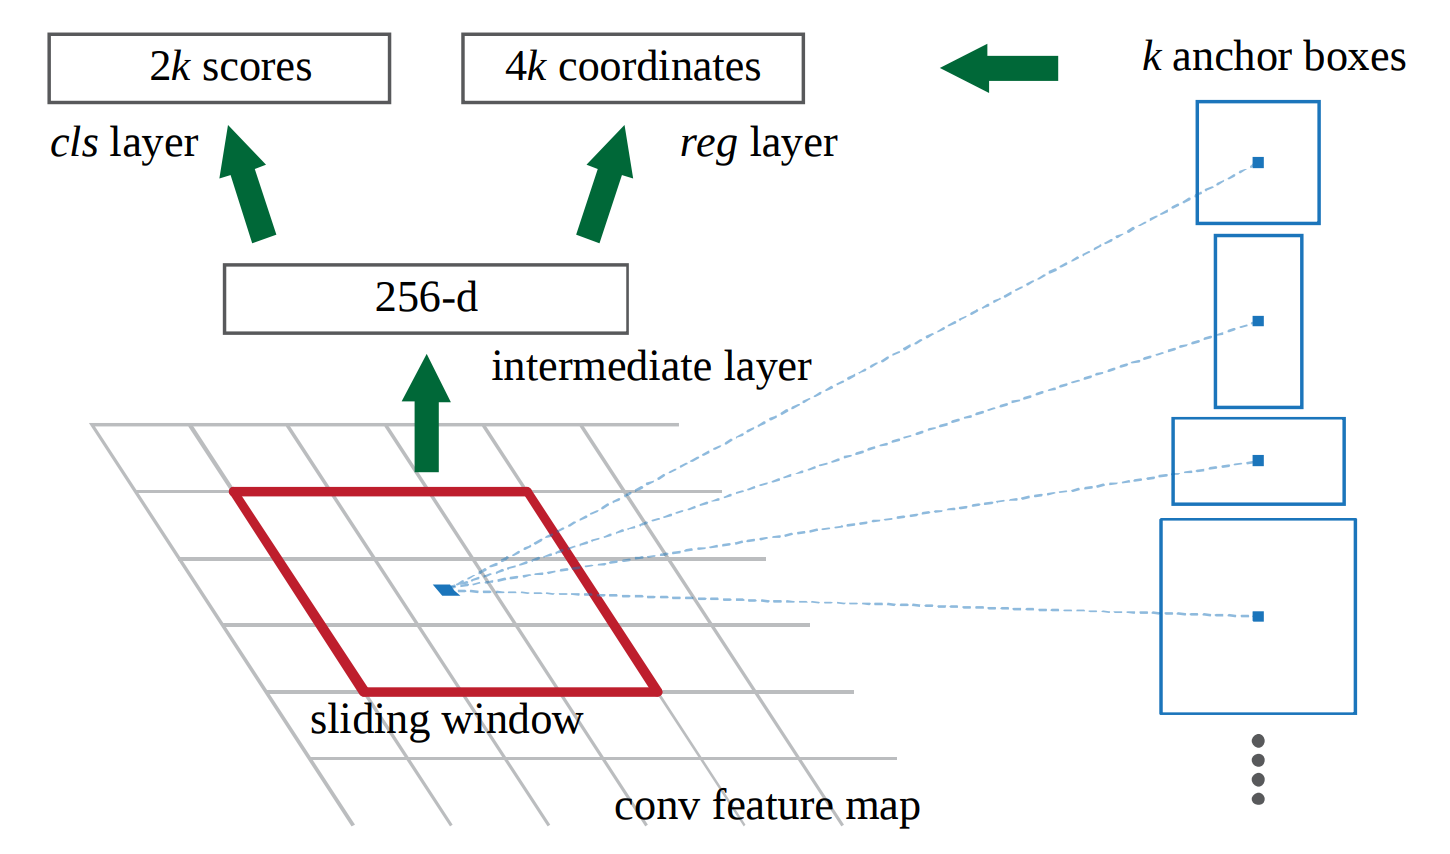
\includegraphics[scale=.5]{image/anchor.PNG}
%     \end{center}
%     \caption{List of all anchors types}
%     \label{ref_chapter2}
%     \end{figure}
% \end{center}
% Anchor: Với mỗi vị trí sliding window, giải thuật sẽ đưa ra N region proposal. Mỗi region tương ứng một trong N loại anchor ở trên. \\

% Kích thước vật lí của mỗi anchor là khác nhau, từ 0.3 mét cho đến 2 mét. Nếu sử dụng single-scale RPN thì sẽ dự đoán tất cả các bao đóng có cùng receptive field. Nên multi-scale RPN đã cho ra những proposal với kích thước nhỏ, lớn khác nhau. Với những proposal kích thước lớn nó có một lớp pooling để tăng receptive field cho những đối tượng lớn hơn. Ở đây những anchor được chia thành 2 level dựa trên kích thước vật lí của nó và sử dụng một nhánh khác của mạng để đưa ra dự đoán cho chúng.\\

% \begin{center}
%     \begin{figure}[htp]
%     \begin{center}
%      \includegraphics[scale=.5]{image/RPN.PNG}
%     \end{center}
%     \caption{3D amodal region proposal network}
%     \label{ref_chapter2}
%     \end{figure}
% \end{center}

% Kiến trúc: Ảnh trên là cho ta trực quan về kiến trúc của mạng. Bước đi (stride) của lớp convolution cuối cùng là 1 tương ứng 0.1 mét trong 3D. Kích thước bộ lọc là 2x2x3 cho level 1 và 5x5x5 cho level 2, chúng tương ứng với 0.4$m^3$ receptive field cho level 1 của những anchor và 1$m^3$ cho level 2 của những anchor lớn hơn.\\

% Với độ phân giải, phạm vi và kiến trúc của mạng thì tổng số anchor là 1,387,646. Trung bình có $92.2\%$ số anchor là rỗng , nó sẽ tự động bị bỏ qua trong quá trình huấn luyện và kiểm tra.\\

% 3D box regression: Mỗi 3D box được biểu diễn tâm điểm của nó $[c_x,x_y,c_z]$ và kích thước của bao đóng là $[s_1,s_2,s_3]$ theo 3 hướng chính của bao đóng. Để huấn luyện 3D box regressor, chúng ta sẽ đoán sự sai biệt của tâm và kích thước giữa anchor và ground truth box. Với mỗi anchor là mẫu dương và grouth truth tương ứng của nó, biễu diễn độ dời của tâm là sự sai biệt $[\Delta c_x,\Delta c_y,\Delta c_z]$ so với hệ tọa độ của máy ảnh. Với sự sai biệt về kích thước thì ta tính độ dời $[\Delta s_1,\Delta s_2, \Delta s_3]$ . Vậy mục tiêu của 3D box regression là một vector có 6 thành phần như sau $ t = [\Delta c_x,\Delta c_y,\Delta c_z,\Delta s_1,\Delta s_2, \Delta s_3]$
% \subsection{Joint Amodal Object Recognition Network}
% \begin{center}
%     \begin{figure}[htp]
%     \begin{center}
%      \includegraphics[scale=.5]{image/ORN.PNG}
%     \end{center}
%     \caption{Joint object recognition network}
%     \label{ref_chapter2}
%     \end{figure}
% \end{center}
%  Sau khi có được những 3D proposal box, không gian 3 chiều cùng với mỗi bao đóng sẽ được cho vào Object Recognition Network (ORN). Theo cách này, những proposal là những bao đóng mà đối tượng nằm hoàn toàn trong đó, ORN có thể vẫn nhận ra kích thước đầy đủ của đối tượng dù có bị ẩn hay dữ liệu bị nhiễu hặc mất mát.\\
 
% 3D ORN: Tất cả các lớp pooling là $2^3$  với stride 2. Với 3 lớp convolution, kích thước của cửa sổ là $5^3$,$3^3$ và $3^3$ tất cả đều có stride là 1. Giữa các lớp fully connected là lớp ReLu và dropout ( hệ số dropout là 0.5).\\

% 2D ORN: Với mỗi 3D proposal box, chúng ta sẽ chiếu những điểm trong proposal box thuộc không gian 3 chiều sang mặt phẳng của ảnh 2 chiều, và lấy bao đóng 2D chứa tất cả những điểm của phép chiếu. Sử dụng mạng VGGnet\cite{VGG} đã huấn luyện sẵn trên ImageNet để trích xuất đặc trưng màu sắc từ ảnh. \\

% 2D và 3D joint recognition: Xây dựng sự kết hợp giữa mạng 2D và mạng 3D để sử dụng cả thông tin về màu sắc và độ sâu. Đặc tính từ VGG Net và 3D ORN sẽ được tổng hợp lại thành một vector đặc tính và cho vào lớp fully connected để giảm số chiều xuống. 2 lớp fully connected sau sẽ lấy kết quả đó để dự đoán nhãn của đối tượng và bao đóng 3D. \\


% \subsection{Kết quả}
% \begin{center}
%     \begin{figure}[H]
%     \begin{center}
%      \includegraphics[scale=.5]{image/table3.PNG}
%     \end{center}
%     \caption{Comparison on 3D object detection}
%     \label{ref_chapter2}
%     \end{figure}
% \end{center}

% Hình 2.4 cho thấy so sánh với 2 phương pháp khác 3D sliding shapes\cite{ss} 
% và 2D Depth-RCNN\cite{guppta}. Kết quả cho thấy sự cải thiện rõ rệt trên tập dữ liệu NYUv2.\\

% \section{DengCVPR 2017\cite{amodal3dobject}}
%  Đây là một công trình gần đây đạt được kết quả khá tốt trong năm 2017 và hứa hẹn sẽ có nhiều cải tiến trong tương lai.\\

% Công trình này nhìn bài toán nhận diện vật thể 3D từ góc nhìn 2D. Một đề xuất mới với mạng neuron nhận diện 3D dựa trên Fast-RCNN\cite{fastrcnn} nó sẽ kết hợp một cách tự nhiên thông tin độ sâu tương ứng với thông tin trên ảnh màu để xác định loại vật thể, hướng và kích thước vật lí. Tại đó bao đóng 2D cùng với ảnh độ sâu sẽ là input.\\



% Nhóm sẽ trình bày chi tiết hơn về công trình này trong phần hướng tiếp cận còn sau đây là những kết quả đạt được của nó. Những thí nghiệm thực hiện trên tập dữ liệu NYUv2 được so sánh với kết quả của deep sliding shape có 19 loại đối tượng khác nhau. Kết quả cho thấy phương pháp này cho chỉ số mAP cao hơn là 4.6$\%$

% \begin{center}
%     \begin{figure}[H]
%     \begin{center}
%      \includegraphics[scale=.5]{image/table4.PNG}
%     \end{center}
%     \caption{Comparison with deep sliding shape}
%     \label{ref_chapter2}
%     \end{figure}
% \end{center}


 


 